%TODOS FOR THIS LAB
%1.  Maybe merge mst and ImgSegMST

\lab{Algorithm}{Kruskal's and Prim's Algorithm}{Kruskal's and Prim's Algorithm}
\label{Ch:Kruskal}

\objective{Find a minimum spanning tree for a connected, weighted graph using Kruskal's Algorithm and Prim's Algorithm.}

\section*{Weighted Graphs and Spanning trees}

Remember that a graph is composed of two sets: a set of nodes and a set of edges that connect the nodes.

\begin{figure}[H]
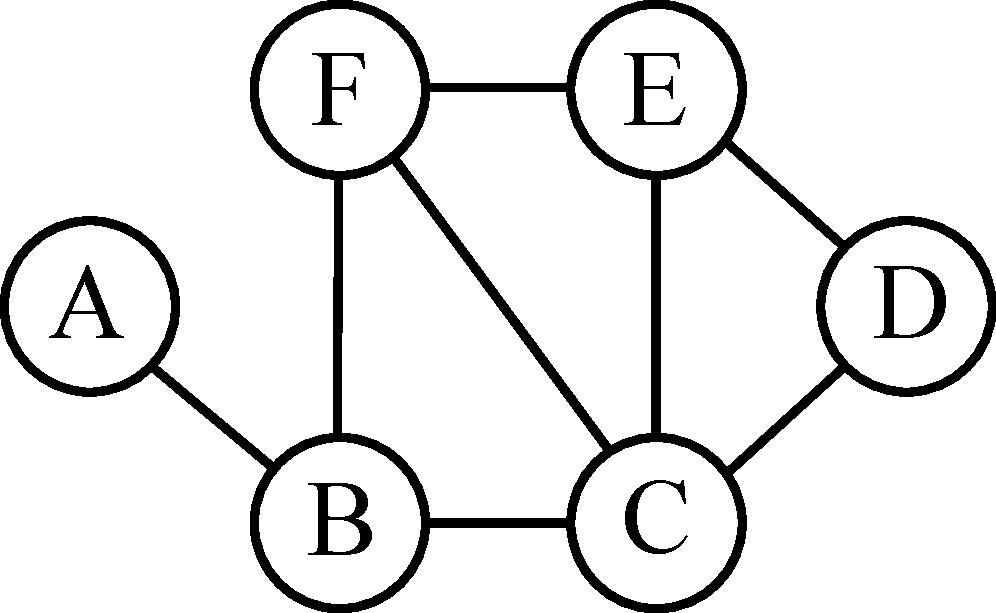
\includegraphics[width = .4\textwidth]{graph1.pdf}
\caption{An example of an undirected graph}
\label{mst:graph1}
\end{figure}

A graph is directed if connections are uni-directional.
A graph is undirected if connections are bi-directional.
Figure 7.1 shows an example of an undirected graph.
A weighted graph is a graph where each edge has a value associated with it.
Usually these values represent some sort of cost or distance.
A connected graph is a graph where there is a path, or a set of edges, that connects every two nodes together.
We can write a matrix that describes this type of graph.
Each row of our matrix represents a starting point and each column represents a destination.
If an edge from one node to another exists, we put the weight of the edge.
If there is no edge, we put a 0.
For the above graph in Figure 7.1 we generate the following matrix:

\[
A = \begin{pmatrix}
0 & 1 & 0 & 0 & 0 & 0\\
1 & 0 & 1 & 0 & 0 & 1\\
0 & 1 & 0 & 1 & 1 & 1\\
0 & 0 & 1 & 0 & 1 & 0\\
0 & 0 & 1 & 1 & 0 & 1\\
0 & 1 & 1 & 0 & 1 & 0\\
\end{pmatrix}
\]

This matrix is called an adjacency matrix.
Note that since the graph is undirected, then this matrix is symmetric.
Now consider the graph in Figure 7.4.  This graph is the same as the graph in Figure 7.1, except now there is a weight attached to each edge.  The matrix for this graph is
\[
A = \begin{pmatrix}
0 & 3 & 0 & 0 & 0 & 6\\
3 & 0 & 5 & 0 & 0 & 4\\
0 & 5 & 0 & 1 & 1 & 5\\
0 & 0 & 1 & 0 & 2 & 0\\
0 & 0 & 1 & 2 & 0 & 4\\
6 & 4 & 5 & 0 & 4 & 0\\
\end{pmatrix}
\]

Another way to store the information from a graph is to make a list of the edges with their corresponding weights.
For an unweighted, undirected graph, this would just mean making a list of the pairs of nodes that correspond to each edge.
For a weighted, undirected graph, a third value could be added to the end of each edge representing the corresponding weight of that edge.
A list like this for the graph in Figure 7.1 would look like this:

\begin{align*}
[('A', 'B'),
 ('B', 'C'),
 ('B', 'F'),
 ('C', 'D'),\\
 ('C', 'E'),
 ('C', 'F'),
 ('D', 'E'),
 ('E', 'F')]
\end{align*}

For this lab, we will be focusing on undirected, weighted graphs.

A spanning tree of a connected, undirected graph $G$ is an undirected graph that contains all the nodes of $G$, a subset of the edges, and no cycles.
A cycle, for undirected graphs, is a path where you start and end on the same node without crossing any edge more than once.
The red in Figure 7.2 is an example of a cycle in an undirected graph.

\begin{figure}[H]
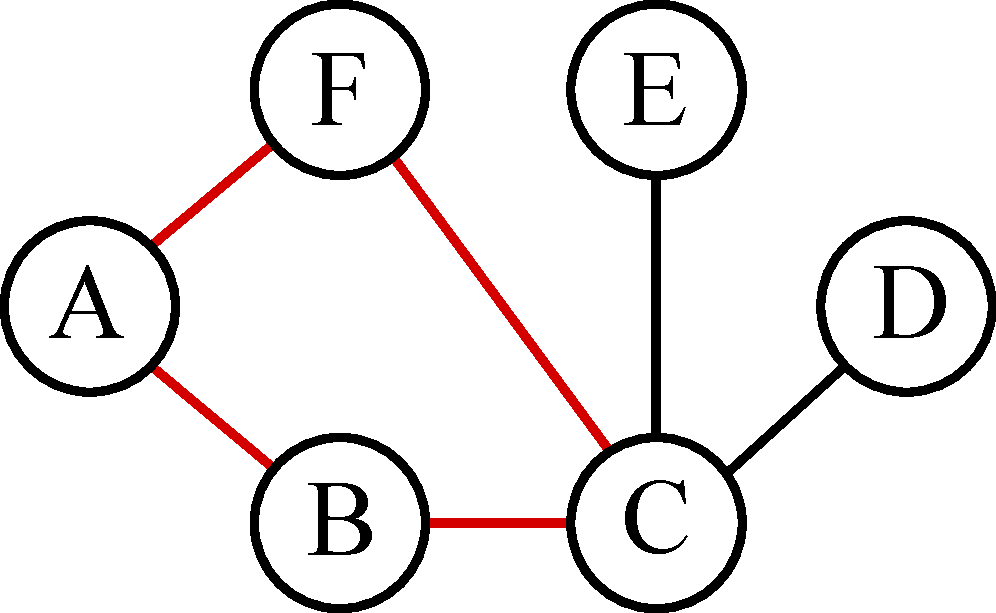
\includegraphics[width = .4\textwidth]{graph3.pdf}
\caption{A cycle in an undirected graph}
\label{mst:graph3}
\end{figure}

The minimum spanning tree (MST) of a weighted, undirected graph is a spanning tree where the total weight is less than or equal to the total weight of every other spanning tree.
Both Kruskal's and Prim's Algorithms are methods that find the minimum spanning tree of a weighted, undirected graph.
Figure 7.3 shows a spanning tree of the graph shown in Figure 7.1.
Figure 8.5 shows a minimum spanning tree of the graph shown in Figure 7.4.

\begin{figure}[H]
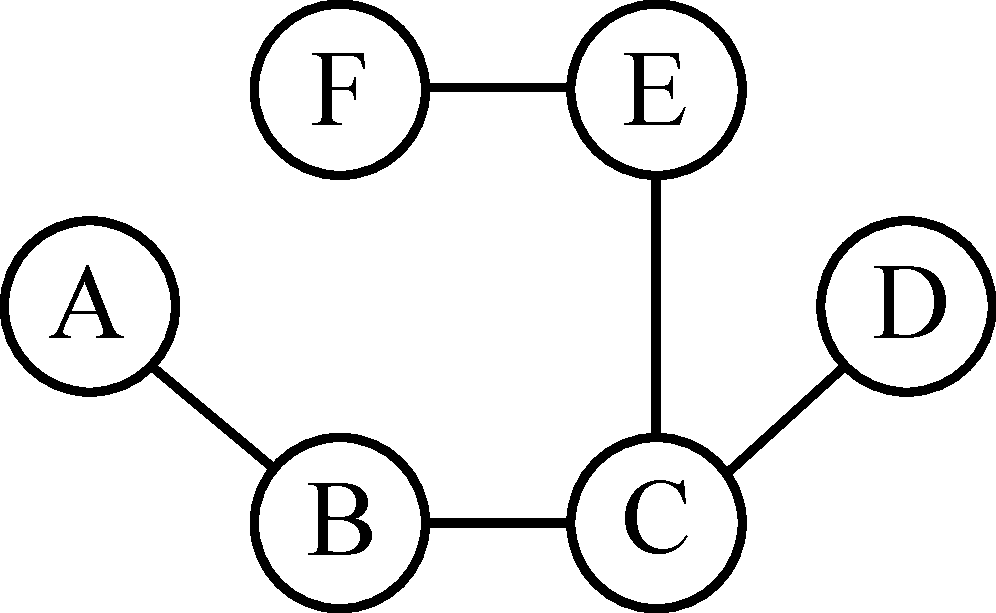
\includegraphics[width = .4\textwidth]{graph2.pdf}
\caption{A spanning tree with no cycles for the graph in Figure 7.1.}
\label{mst:graph2}
\end{figure}

\begin{figure}[H]
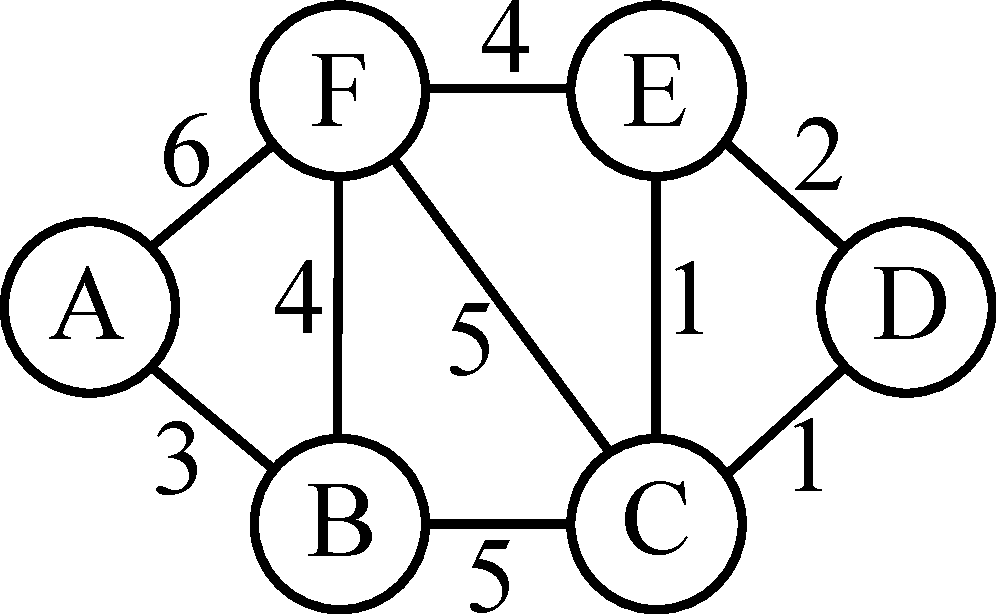
\includegraphics[width = .4\textwidth]{graph4.pdf}
\caption{A weighted, undirected graph}
\label{mst:graph4}
\end{figure}

\begin{figure}[H]
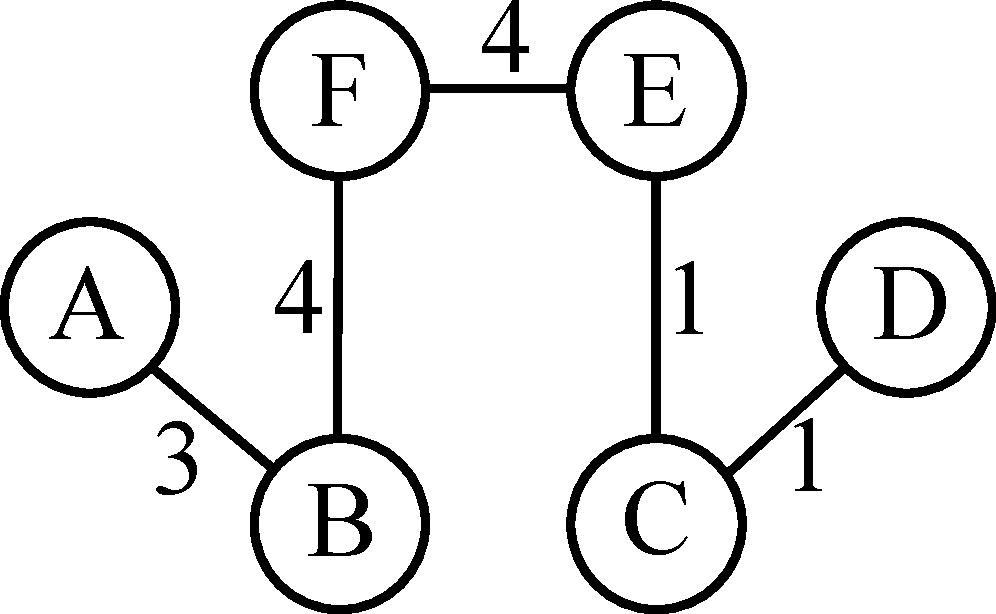
\includegraphics[width = .4\textwidth]{graph5.pdf}
\caption{The MST of the graph in Figure 7.4.}
\end{figure}

\section*{Kruskal's algorithm}

Given a weighted, directed graph G with $n$ nodes, Kruskal's algorithm finds a minimum spanning tree by first sorting the edges from smallest to largest.
Then starting with the smallest, the algorithm adds edges to the tree as long as the addition of each new edge does not create a cycle.
When $n-1$ edges have been added, the algorithm stops.

In order to avoid creating cycles while building the tree, it is necessary to keep track of which portions of the tree currently lie in connected groups.
This can be done by creating a dictionary where, when the algorithm starts, each node points to itself as the "root" of its own tree.
As you add edges to the tree you will change which nodes are the "root" nodes. This tracks which nodes are currently connected.
Doing this allows us to run the algorithm by iterating over the edges by weight in ascending order, and adding them to the tree if they connect nodes which are not already connected by the current tree.

Consider the graph in Figure 7.4 and apply Kruskal's algorithm.
First, we initialize our tree to be an empty list: \li{[]}.
To track the root nodes of each tree, we will also initialize a dictionary where each node points to itself.
It will look like this: \li{\{A:A, B:B, C:C, D:D, E:E, F:F\}}.
Since there are 6 nodes in the graph, we will continue until we have 5 edges in the tree.
Next, sort the edges by weight.
The result is something like the list \li{[(C, D, 1), (C, E, 1), (D, E, 2), (A, B, 3), (B, F, 4), (E, F, 4), (B, C, 5), (C, F, 5), (A, F, 6)]}.

Now we begin iterating through the edges to build the tree.
The first edge in the list is \li{(C,D,1)}.
The root for \li{C} is \li{C} and the root for \li{D} is \li{D}, so we add this edge to the tree.
The tree becomes \li{[(C, D, 1)]}.
We then change the root node of \li{D} to be \li{C}.
The dictionary of root nodes now looks like \li{\{A:A, B:B, C:C, D:C, E:E, F:F\}}.

Now we process the next edge, \li{(C, E, 1)}.
The root node of \li{C} is \li{C}, and the root node of \li{E} is \li{E}, so adding this edge does not create a cycle.
We add this edge into the tree, so the tree is now \li{[(C, D, 1), (C, E, 1)]}.
Then we change the root of \li{E} so that it is \li{C}, so the dictionary is \li{\{A:A, B:B, C:C, D:C, E:C, F:F\}}.

The next edge is \li{(D, E, 2)}.
The root node of the tree containing \li{D} is \li{C} and the root node of the tree containing \li{E} is \li{C}, so these nodes are already connected, so we do not add this edge to the tree.

The next edge is \li{(A, B, 3)}.
The root node for \li{A} is \li{A}, and the root node for \li{B} is \li{B}, so we add the edge to the tree and update the dictionary.
The dictionary becomes \li{\{A:A, B:A, C:C, D:C, E:C, F:F\}}

The next edge is \li{(B, F, 4)}.
The root node for \li{B} is \li{A} and the root node for \li{F} is \li{F}, so we add the edge to the tree and change the root node of \li{F} to be \li{A}.
The dictionary becomes \li{\{A:A, B:A, C:C, D:C, E:C, F:A\}}

The next edge is \li{(E, F, 4)}.
The root node for \li{E} is \li{C} and the root node for \li{F} is \li{A}.
We add the edge to the tree and end the algorithm since there are now 5 edges in the tree.
(If we were to continue the algorithm, we would update the root node of \li{A} to be \li{C}.)

Notice how we updated the root of the root node to one of the nodes in the edge added.
We manage the root nodes in this manner in order to find the root node by tracing back through the dictionary until we find a node that points to itself.
For example, to find the root node of \li{F} we first need to get the value for \li{F} from the dictionary.  This is \li{A}.
Then we get the value for \li{A} from the dictionary which is \li{C}.
Since the value of \li{C} in the dictionary is itself, the \li{C} is the root node of the graph containing \li{F}.
It is necessary to trace through the dictionary in this manner each time because we avoid iterating over all of the nodes and updating their root values everytime.

Below is the pseudocode for the algorithm as we have described it above:

\begin{itemize}

% Note: The comments in the solutions match the pseudocode.
% When making changes, please keep that in mind.

\item Initialize an empty list of edges for the minimum spanning tree.

\item Make a dictionary that points each node toward its root (not always directly to it).
Start with each node pointing to itself.

\item Initialize the number of nodes that still need to be processed to the number of nodes minus 1.

\item Define a helper function that, given a node, traces through the dictionary to find the root of its tree.
This can be done like this:

	\begin{itemize}

	\item Initialize a temporary variable to be the node for which we are finding the root.

	\item While the temporary node does not point to itself in the dictionary:

		\begin{itemize}

		\item Update the temporary node to be the node it currently points to in the dictionary.

		\end{itemize}

	\item Return the temporary node.

	\end{itemize}

\item Iterate over the edges by ascending weight.
Use a \li{for} loop for this and return the tree when it is big enough which breaks the loop for you.

	\begin{itemize}

	\item Trace through the dictionary to find the root node of each of the nodes in the edge you are processing.

	\item If the roots are not the same (i.e. if adding the edge doesn't form a cycle):

		\begin{itemize}

		\item Add the edge to the tree.

		\item Lower the number of edges remaining by one.

		\item If the number of edges remaining is 0, return the tree (which also breaks the loop).

		\item Update the root of the root of the second node in the edge to be the root of the first node in the edge.
			This lets us record that the two subtrees are now connected.

		\end{itemize}

	\end{itemize}

\end{itemize}
Note on implementation: You can iterate over a sorted copy of a list using the built in \li{sorted} function.
You can sort by the third value in each tuple using the \li{itemgetter} function that is part of the \li{operator} library included with Python.
For example:
\begin{lstlisting}
from operator import itemgetter
...
for n1, n2, weight in sorted(edges, key=itemgetter(2)):
    ...
\end{lstlisting}

\begin{problem}
Implement Kruskal's algorithm.
Test your algorithm on random symmetric arrays.
You can generate a random symmetric array by multiplying a random array by its transpose.
Use the data from MSTdata.npy to test your tree.
Use np.load("MSTdata.npy") to get it.
Use the \li{formChanger} function below to put it in the right form.
\begin{lstlisting}
def formChanger(oldData):
    newData=[]
    for i in oldData: newData.append((i[0],i[1],int(i[2])))
    return newData
\end{lstlisting}
\end{problem}
\section*{Prim's algorithm}

Prim's is a similar algorithm for finding minimum spanning trees.
While it is much slower than Kruskal's algorithm for sparse graphs, it is much faster for dense graphs because Prim's algorithm avoids sorting the edges.

Again, consider the example shown in Figure 7.4.
We first initialize a dictionary with all the nodes as keys in order to track which nodes have not been processed.
At the beginning it will be \li{\{A:False, B:False, C:False, D:False, E:False, F:False\}}.
We then form the dictionary that maps each node to the edges that contain it.
Since we will already know one node of each edge while we use the dictionary, we only need to store the node that is not being looked up.
It should end up looking like \li{\{A:[(B, 3), (F, 6)], B:[(A, 3), (C, 5), (F, 4)], C:[(B, 5), (D, 1), (E, 1), (F, 5)], D:[(C, 1), (E, 2)], E:[(C, 1), (D, 2), (F, 4)], F:[(A, 6), (B, 4), (C, 5), (E, 4)]\}}.
We will also initialize an empty dictionary to track the shortest edges that run between nodes we have processed and nodes that we haven't.
As we iterated over the edges in our initialization step, we are also able to find the shortest edge.
In this case, it is \li{(D, C, 1)}.
Let's start with \li{(D, C, 1)} and initialize our tree as the list \li{[(D, C, 1)]}.
Next, we mark \li{D} and \li{C} as processed in the dictionary that tracks which nodes have been processed.
We now start to build our dictionary of nodes that are one edge away from our processed nodes.
In this case, after adding the shortest edges between processed and unprocessed nodes to the dictionary, the dictionary becomes \li{\{B:(C, B, 5), E:(C, E, 1), F:(C, F, 5)\}}.
Notice we did not include \li{E:(D, E, 2)} because there is a shorter edge to \li{E} from \li{C}.

Of the edges in the dictionary of edges that can be processed next, the shortest is \li{(C, E, 1)}, so we add that edge to the tree and mark \li{E} as processed.
With \li{E} being processed, we can now reach \li{F} at a cost of 4.
After making this change, the dictionary of edges to process becomes \li{\{B:(C, B, 5), E:(C, E, 1), F:(E, F, 4)\}}.
Since \li{E} no longer needs to be processed, we can remove it from consideration.
So this dictionary now becomes \li{\{B:(C, B, 5), F:(E, F, 4)\}}.

Of the edges to be processed next, \li{(E, F, 4)} is the shortest, so we add it to the tree and mark \li{F} as processed.
After performing the appropriate modifications to the dictionary of edges to be processed next, it becomes \li{\{B:(F, B, 4), A:(F, A, 6)\}}.

Of the edges to be processed next, \li{(F, B, 4)} is the shortest, so we add it to the tree and mark \li{B} as processed.
After performing the appropriate modifications to the dictionary of edges to be processed next, it becomes \li{\{A:(B, A, 3)\}}.

The only edge to be considered is \li{(B, A, 3)}, so we add it to the tree.
The tree is long enough that it it spans the nodes, so the algorithm is finished.

Here's pseudocode for a version of Prim's algorithm.
While it is not a perfectly optimized version, it is pretty good.

\begin{itemize}

% Note: The comments in the solutions match the pseudocode.
% When making changes, pleas keep that in mind.

\item Initialize a dictionary to track which nodes have been processed.

\item Initialize an empty dictionary of lists to track the edges containing each node.

\item Fill the edge list.
	Be sure to add each edge to the list corresponding to both of its nodes.

\item Get the first edge to add (The shortest edge from any given node is a good pick).

\item Mark the nodes in the first edge as processed.

\item Initialize the tree to be the list containing the first edge.

\item Initialize an empty dictionary that will be used to contain the edges that can be processed next.

\item Define a helper function to insert an edge into the dictionary (if that insertion is needed).
	This can be done as follows:

	\begin{itemize}

	\item Get the value of the node that is reached by the edge.

	\item If that node isn't in the dictionary, set its value to be the edge passed to the functions.

	\item If it is in the dictionary already, set its value to be the shorter of the edges being processed and the edges already in the dictionary.

	\end{itemize}

\item Use the helper function to insert the edges reached by the first two processed nodes into the dictionary of edges to be processed.

\item Until the tree contains enough edges to span all the nodes:

	\begin{itemize}

	\item Find the shortest edge in the dictionary of edges to be processed.

	\item Remove the shortest edge from the dictionary.

	\item Add it to the tree.

	\item Mark the node reached by the new edge as processed.

	\item Use the helper function to insert the edges reached by the newly processed node into the dictionary of edges to be processed.

	\end{itemize}

\item Return the completed tree.

\end{itemize}

\begin{problem}
Write a Python function that uses Prim's algorithm to find the minimum spanning tree of a graph.
Test your implementation with the same data as the previous problem.
Compare the speed of Prim's algorithm with the speed of Kruskal's algorithm.
Create a function which prints these two times.
\end{problem}

Many graph packages have functions for finding the minimal spanning tree. One of these is NetworkX. You begin as follows
\begin{lstlisting}
import networkx as nx
G=nx.Graph()
\end{lstlisting}
You can add a node $x$ with \li{G.add_node(x)} and add a edge from $x$ to $y$ with weight n with \li{G.add_edge(x,y,weight=n)}. Then \li{nx.minimum_spanning_tree(G)} returns the minimal spanning tree using Kruskals algorithm.

\begin{problem}
Use NetworkX to find the minimal spanning tree of the data in MSTdata.npy.
Compare the output with that of your algorithm.
Create a function which prints your comparison.
\end{problem}

%Add specifications

\section*{Image Segmentation}

%Lab \ref{MSTImgSeg}

One application of Minimal Spanning Trees (MSTs) is image segmentation.
Kruskal's algorithm is especially good at this.
You can convert an image into graph. Each pixel is a vertex and you define weights between the nodes. You then build the minimal spanning tree. If you take away the edge with the greatest weight you will get two forests (removing an edge from any graph with no cycles will create two forests). Then you can continue doing this to each forest to split up those forests. Each forest corresponds to a segment of the image.
Let $k$ be the number of divisions that is wanted and $n$ be the number of nodes.
Kruskal's algorithm is performed until $n-(k+1)$ edges are added which is the same as taking out the $k$ edges with greatest weights.

There are many different ways to turn an image into a graph and weight the edges.
A simple, yet effective, version is to make every pixel a node and the edges are the difference in intensities in the four cardinal directions.


This means that there are less than $4n$ edges.
Other image segmentation algorithms have to use $n^2$ space.
This gives the MST algorithm a critical advantage over other image segmentation algorithms.

\begin{problem}
Write a function that takes a black and white image as input and outputs a list of the edges and a list of nodes.
Store the edges using the form \li{(node,node,weight)}.
\end{problem}

The provided Kruskal's algorithm takes as inputs the list of nodes, the list of edges and the number of divisions desired.
The number of divisions often has to be higher than the actual number that is needed because sometimes one or two pixels form a division because the difference between them and the pixels around them is so great.
You will have to adjust the number of divisions until the desired result is found.  See Figure 9.1.

\begin{problem}
Perform the image segmentation algorithm on the image, then graph the original image and the three largest divisions.
(Use the Counter class from collections to find the number of pixels in each division.)
\end{problem}

\begin{problem}
Make a division of the image a different color.
\end{problem}


\vfill
\begin{figure}[ht]
\begin{minipage}[b]{0.47\linewidth}
\centering

\includegraphics[width=\textwidth]{MSTseg1.jpg}
\end{minipage}
\hspace{0.5cm}
\begin{minipage}[b]{0.47\linewidth}
\centering

\includegraphics[width=\textwidth]{MSTseg2.jpg}
\end{minipage}
\begin{minipage}[b]{0.47\linewidth}
\centering

\includegraphics[width=\textwidth]{MSTseg3.jpg}
\end{minipage}
\hspace{0.5cm}
\begin{minipage}[b]{0.47\linewidth}
\centering

\includegraphics[width=\textwidth]{MSTseg4.jpg}
\end{minipage}
\caption{The original image is in the top left hand corner. The three larges segments are shown in the other corners. The original image was 498x498 and 50000 divisions were used.}
\end{figure}
\vfill 
